\chapter{Image filtering option}

%-------------------------------------------------------------------
%-------------------------------------------------------------------
%-------------------------------------------------------------------

\section{Generalities }

\subsection{Introduction }
MicMac is not an image processing tool, but for doing its photogrammetric
work it requires image processing at different part. The image processing
is mainly done by the "ElIsE" library, described in the document {\tt "doc\_elise.pdf"}
which is distributed in the same folder than this documentation.
The   "ElIsE" library is relatively large library and contains much
more option than what is really usefull in MicMac and it appears
that it may interesting for some user to user access, in commande
line form, without using \CPP, to some filtering option of  "ElIsE" .


Also several command were historically existing, it has been unified
and what is described here is done using a unique command 
{\tt Nikrup}  \footnote{this name refers to the "invert polish like" syntax used}:

\begin{verbatim}
>mm3d Nikrup
*****************************
*  Help for Elise Arg main  *
*****************************
Mandatory unnamed args : 
  * string :: {Expression}
  * string :: {File for resulta}
Named args : 
  * [Name=Box] Box2di :: {Box of result, def computed according to files definition}
  * [Name=NbChan] INT :: {Number of output chan, def 3 if input %3, else 1}
  * [Name=Type] string :: {Type of output, def=real4 }
\end{verbatim}

The two main parameter are :

\begin{itemize}
   \item a "mathematicall" expression that describes the image to create, this expression is
        done using the so named  invert polish notation
   \item a file where write this result.
\end{itemize}

Also it may seems very basic, it's possible to create relatively complicate
operation due to the functionnal aspect of the "language".  Two example :


\begin{verbatim}
mm3d Nikrup "* 128 + 1 cos + * Y 0.2 * 0.06 * X cos * 0.06 X" Test.tif Box=[0,0,400,400] Type=u_int1

mm3d Nikrup "+ * 2 =F > Crop-Therm.tif 160 close @F 5711  80 " Test.tif Type=u_int1
\end{verbatim}



\begin{figure}
\begin{center}

\includegraphics[width=45mm]{ImNikrup/Sin.jpg}
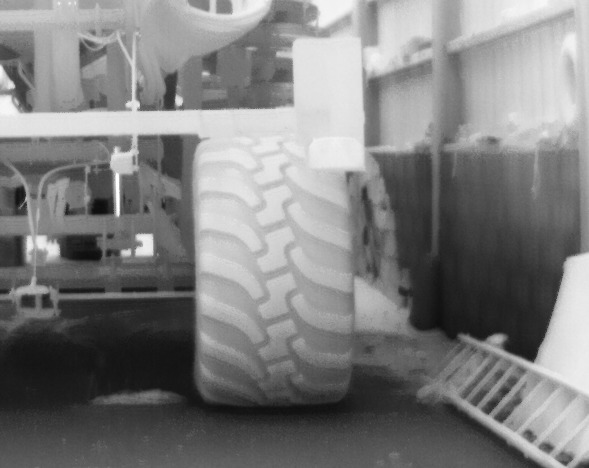
\includegraphics[width=45mm]{ImNikrup/CropTrac.jpg}
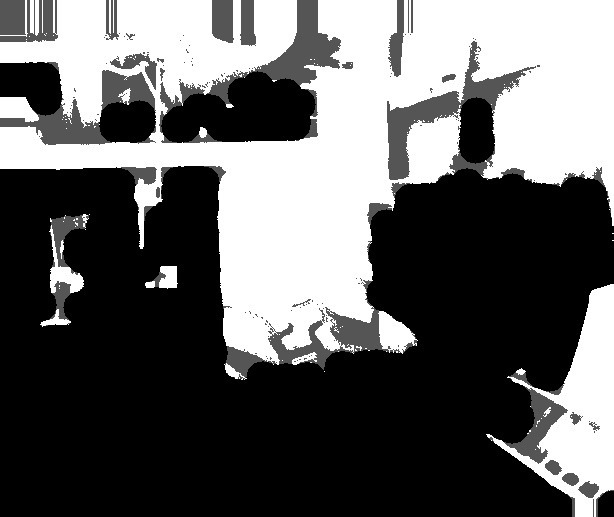
\includegraphics[width=45mm]{ImNikrup/CloseTrac.jpg}
\end{center}
\caption{Image with sinus formula, initail Crop-Therm.tif, result of closing}
\label{FIG:Nikrup1}
\end{figure}


The result of the two formula are presented on figure~\ref{FIG:Nikrup1}. The
infix notation may be strange for user not familiar with post-script of lisp or
any other infix language. To be honest, this notation is more done to be 
written than to be read  \dots However, the notation accept parenthesis,
in most case they will superflous but may help the edition, for example
$+ a * b c$ is strictlty equivalent to $+ a (* b c)$ or $(+ a (* b c))$.
When operaror have optionnal number of argument, parenthesis become
mandatory when you want to use it more than the minimal number; for
example $*$ and $+$ has any number of argument over $2$, but if you
write $+ a  b c$ , $c$ would be ignored and will generate an error ;
you must write $(+ a b c)$ (which in this particular case is equivalent to $+ a + b c$).

The above example  illustrate the use of parenthesis with a formula equivalent to previous one :


\begin{verbatim}
mm3d Nikrup "(* 128 (+ 1 (cos + (* Y 0.2) (* 0.06  X (cos * 0.06 X)))))" Test.tif Box=[0,0,400,400] Type=u_int1
\end{verbatim}

Using the {\tt Nikrup} tool is essentially a matter of creating mathematical expression, which can be
atomic (terminal) expression or the application of an operateur to  one or several other expression.

\subsection{Formalism }

The mathematicall object manipulated by expression, are simply
function $\mathbb{R}^k  \rightarrow  \mathbb{R}^p $.

For now it is restricted to $\mathbb{R}^2  \rightarrow  \mathbb{R}^p $, but
could easily be generalized as {\tt ElIsE} support the general case.



%==============================================================

\section{Atomic expression}

Atomic expression are expression that are created without requiring other expression.

\subsection{constant}

Constant are integer or real. They correspond to the following regular expression :

\begin{itemize}
   \item  {\tt "-?[0-9]+"} for integer;
   \item  {\tt "-?[0-9]+\textbackslash.[0-9]*"} for real;
\end{itemize}

They correspond to a constant funtion $\mathbb{R}^2  \rightarrow  \mathbb{R}$.

\subsection{Existing images}

For any expression finish by  {\tt tif,tiff,jpg,jpeg,arw,cr2} , a file
must exist, the expression will be interpreted as  the function
that associate to each point the value stored in the file.

Typically it will be $\mathbb{R}^2  \rightarrow  \mathbb{R}$ for gray level image
and $\mathbb{R}^2  \rightarrow  \mathbb{R}^3$ for a $rgb$ image.

\subsection{Coordinates}

The coordinate expression are $\mathbb{R}^2  \rightarrow  \mathbb{R}$  correspond to :

\begin{itemize}
   \item  $X : (x,y) \rightarrow x$
   \item  $Y : (x,y) \rightarrow y$
   \item the expression $Xk$, prepar a genaralization to any dimension $Xk : (x_1,x_2, \dots x_p)  \rightarrow  x_k$;
         typically $X0$ correspond tp $X$ and $X1$ to $Y$;
\end{itemize}

%==============================================================

\section{Mathematicall operator}

Classically, for any mathematical operator $\odot : \mathbb{R}^n  \rightarrow  \mathbb{R}$,
we can define an operator on funcion   $(\odot f_1 \dots f_n) (x) = (\odot f_1(x) \dots f_n(x)) $.

\subsection{unary}

The unary operator are :

\begin{itemize}
   \item {\tt u-}  for unary minus;
   \item {\tt !}  for logical negation;
   \item {\tt \textasciitilde}  for bit to bit negation
   \item {\tt signed\_frac}  is the fractionnal part ($\in ]-\frac{1}{2},\frac{1}{2}]$),  {\tt ecart\_frac} is
         its absolute value;
   \item trigonometric function {\tt cos, sin, tan, atan};
   \item exponential and log {\tt log,log2,exp};
   \item square, cube and root {\tt square,cube,sqrt};
   \item the error function {\tt erfcc}  $ erfcc(x) =  1-{\frac {2}{\sqrt {\pi }}}\int _{x}^{\infty }e^{-t^{2}}$;
\end{itemize}


\subsection{binary}
The binary operator are :

\begin{itemize}
   \item aritmetic {\tt -, /, \%, mod}  , {\tt \%} is C-like modulo, {\tt mod} is the mathematical modulo;
   \item {\tt pow} for $x^y$;
   \item comparison {\tt >, >=, <, <=, ==, !=} (C-like: {\tt ==}  equal, {\tt !=} not equal);
   \item logical combinaison : {\tt \&\&} and,   {\tt ||} or;
   \item bit to bit  combinaison : {\tt \&} and,   {\tt |} or , {\tt \^{}} exclusive or;
   \item bit shift {\tt >>} and {\tt <<} .

\end{itemize}


\subsection{ternary}

There is one ternary operator {\tt ?}. $? f_1 f_2 f_3$ is the function that
return $f_2(x)$ if $f_1(x)$ is true (non zero) and else $f_3(x)$.

\subsection{associative}

There is $4$ associative operator {\tt +,*,min,max} , they accept between $2$ and infinity number of parameter.
With more than two parameter the parenthesis must be used.

%==============================================================

\section{Morphological filter}

Morphological filter use a chamfer distance as parameters, here are
the $4$ distance, corresponding to more or less precise approximation of
euclidean distance, and their name :

\begin{itemize}
   \item {\tt 4} : the $4$ neigboor distance;
   \item {\tt 8} : the $8$ neigboor distance;
   \item {\tt 32} : distance were $4$ neigboor value $2$, and diagonal value $3$;
   \item {\tt 5711} : distance were $4$ neigboor value $5$, and diagonal value $7$, and $2,1$ neigboor value $11$;
\end{itemize}

\subsection{Extinction function}

Let $I$ be the input function, compute for each pixel where $I(p) \neq 0$ , the
distance to the nearest point where $I(P) = 0$.

Parameters :

\begin{itemize}
   \item   $2$ mandatory the function and the chamfer;
   \item   $1$ optional, the max distance  $D^{max}$ that will be computed,
           this parameter is necessary to fix the size of buffer;
           default = $256$; the pixel would theorically have  a value
           over  $D^{max}$ will have  $D^{max}$.
\end{itemize}

Examples : 

\begin{verbatim}
mm3d Nikrup "extinc >  VisAB070410.tif 32000 5711" Test.tif
mm3d Nikrup "(extinc >  VisAB070410.tif 32000 5711 500)" Test.tif
\end{verbatim}


\subsection{Dilatation and erosion}

The $3$ mandatory parameter are  :

\begin{itemize}
   \item  function
   \item  chamfer
   \item  distance of dilatation (erosion);
\end{itemize}
   
Examples : 

\begin{verbatim}
mm3d Nikrup "(dilate >  VisAB070410.tif 32000 5711 50)" Test.tif
mm3d Nikrup "(erode >  VisAB070410.tif 32000 5711 50)" Test.tif
\end{verbatim}

\subsection{Closure and opening}

Parameters are the same as Dilatation and erosion, with one more
optionnal (def=0) if the  second operation is not exactly the  same
size than the first one.

\begin{verbatim}
mm3d Nikrup "(close >  VisAB070410.tif 32000 5711 50)" Test.tif
mm3d Nikrup "(close >  VisAB070410.tif 32000 5711 50 -10)" Test.tif
\end{verbatim}


%==============================================================

\section{Linear Filter}


\subsection{deriche and polar}

The deriche operator compute the gradient according to cany-deriche algorithm.
The input function must be are $\mathbb{R}^2  \rightarrow  \mathbb{R}$ , and 
the output is  $\mathbb{R}^2  \rightarrow  \mathbb{R}^2$ as it store the 
$\frac{\partial I}{\partial x}$ and $\frac{\partial I}{\partial y}$.
It take $2$ parameters, the function and the size of the multiplier in
the exponent (typically the sigma of the pseudo gaussian filter is invertly
proportionnal to its size).

The polar operator take as input and output a $\mathbb{R}^2  \rightarrow  \mathbb{R}^2$, and
for each pixel it return the module and angle. It can typically be used in 
combinaison with a gradient operator.

\begin{verbatim}
mm3d Nikrup "polar deriche   VisAB070410.tif 1 " Test.tif
\end{verbatim}


\subsection{average}

The operartor {\tt moy} compute the average on a square window, a mandatory parameter 
is the size of the window; an optional parameter is the number of iteration.

\begin{verbatim}
% average on a 13x13 window
mm3d Nikrup "moy VisAB070410.tif  6" Test.tif
% 4 iteration of the  average on a 7x7 window
mm3d Nikrup "(moy VisAB070410.tif  3 4)" Test.tif
\end{verbatim}

%==============================================================

\section{Using symbol}

If the same function is used several time, symbol can be used to avoid
repetetion, it has two benefit : make easier to write, sometime save
computation time at execution. The syntax is :

\begin{itemize}
   \item  {\tt =Symb Func}  to set the symbol {\tt Symb} to {\tt Func}, 
         it returns {\tt Func}
   \item  {\tt @F} to refer to value set ;
   \item  {\tt (=Symb Func Func2) }  to set the symbol {\tt Symb} to {\tt Func} but return {\tt Func2};
\end{itemize}

Let comment previous example :


\begin{verbatim}
mm3d Nikrup "+ * 2 =F > Crop-Therm.tif 160 close @F 5711  80 " Test.tif Type=u_int1
\end{verbatim}

\begin{itemize}
   \item  {\tt =F > Crop-Therm.tif 160} set {\tt F} to the binarizatuon of image {\tt Crop-Therm.tif}
          with threshol $160$
   \item  the value computed is the $2*F+ Close(F)$, so at the end we have :
   \begin{itemize}
          \item  $3$ in F;
          \item  $1$ in point in the closure but not in $F$;
          \item  $0$ in point out of the closure .
   \end{itemize}
\end{itemize}

%==============================================================

\section{Coordinate operator}

   % - - - - - - - - - - - - - - - - - - - - - - - - - - - - - 
\subsection{Permutation}

Permutation operator takes a function and a array of int as parameter.
The following example transform $rgb$ in $bgr$ :

\begin{verbatim}
mm3d Nikrup "permut IMGP7029.JPG [2,1,0]" Test.tif
\end{verbatim}


   % - - - - - - - - - - - - - - - - - - - - - - - - - - - - - 
\subsection{Projection}

The projection operator $vk$, give acces to a given channel.
The following example compute a gray level image from 
rgb by averaging the $3$ channels :


\begin{verbatim}
mm3d Nikrup "(/ (+ (=F IMGP7029.JPG v0 @F) v1 @F v2 @F) 3)" Test.tif
\end{verbatim}

   % - - - - - - - - - - - - - - - - - - - - - - - - - - - - - 
\subsection{Concatenation}

The concatenation operator {\tt ,}  takes $2$ function 
$\mathbb{R}^k  \rightarrow  \mathbb{R}^p $ and
$\mathbb{R}^k  \rightarrow  \mathbb{R}^n $ and return a function
$\mathbb{R}^k  \rightarrow  \mathbb{R}^{n+p}$. Like any
associative operator, it can take any number of parameters .
Following example transform a "rgb" to "bgr" :


\begin{verbatim}
mm3d Nikrup "(, (=F IMGP7029.JPG v2 @F) v1 @F v0 @F)" Test.tif
\end{verbatim}






